% Manuel Lippert - Paul Schwanitz
% Physikalisches Praktikum

% 3.Kapitel  Protokoll

% Variables
\def\skalierung{0.65}

\chapter{Messprotokoll}
\label{chap:protokoll}

Das Messprotokoll wurde am Versuchstag handschriftlich erstellt und hier als
PDF-Datei eingefügt. Dabei wurden Durchführung und Aufbau schon vorher in dieses
Dokument beschrieben, je nachdem.

\section{Versuchsaufbau und Beschreibung}
\label{sec:aufbau}

% Manuel Lippert - Paul Schwanitz
% Physikalisches Praktikum

% 3.Kapitel  Protokoll 

\subsection{Invertiertes Pendel}
\label{sub:aufbauPendel}
% TODO: #24 Aufbau Pendel @ManeLippert

% Manuel Lippert - Paul Schwanitz
% Physikalisches Praktikum

% 3.Kapitel  Protokoll

\subsection{Shinriki-Oszillator}
\label{sub:aufbauShinriki}

\begin{figure}[h]
    \centering
    %TODO #31
    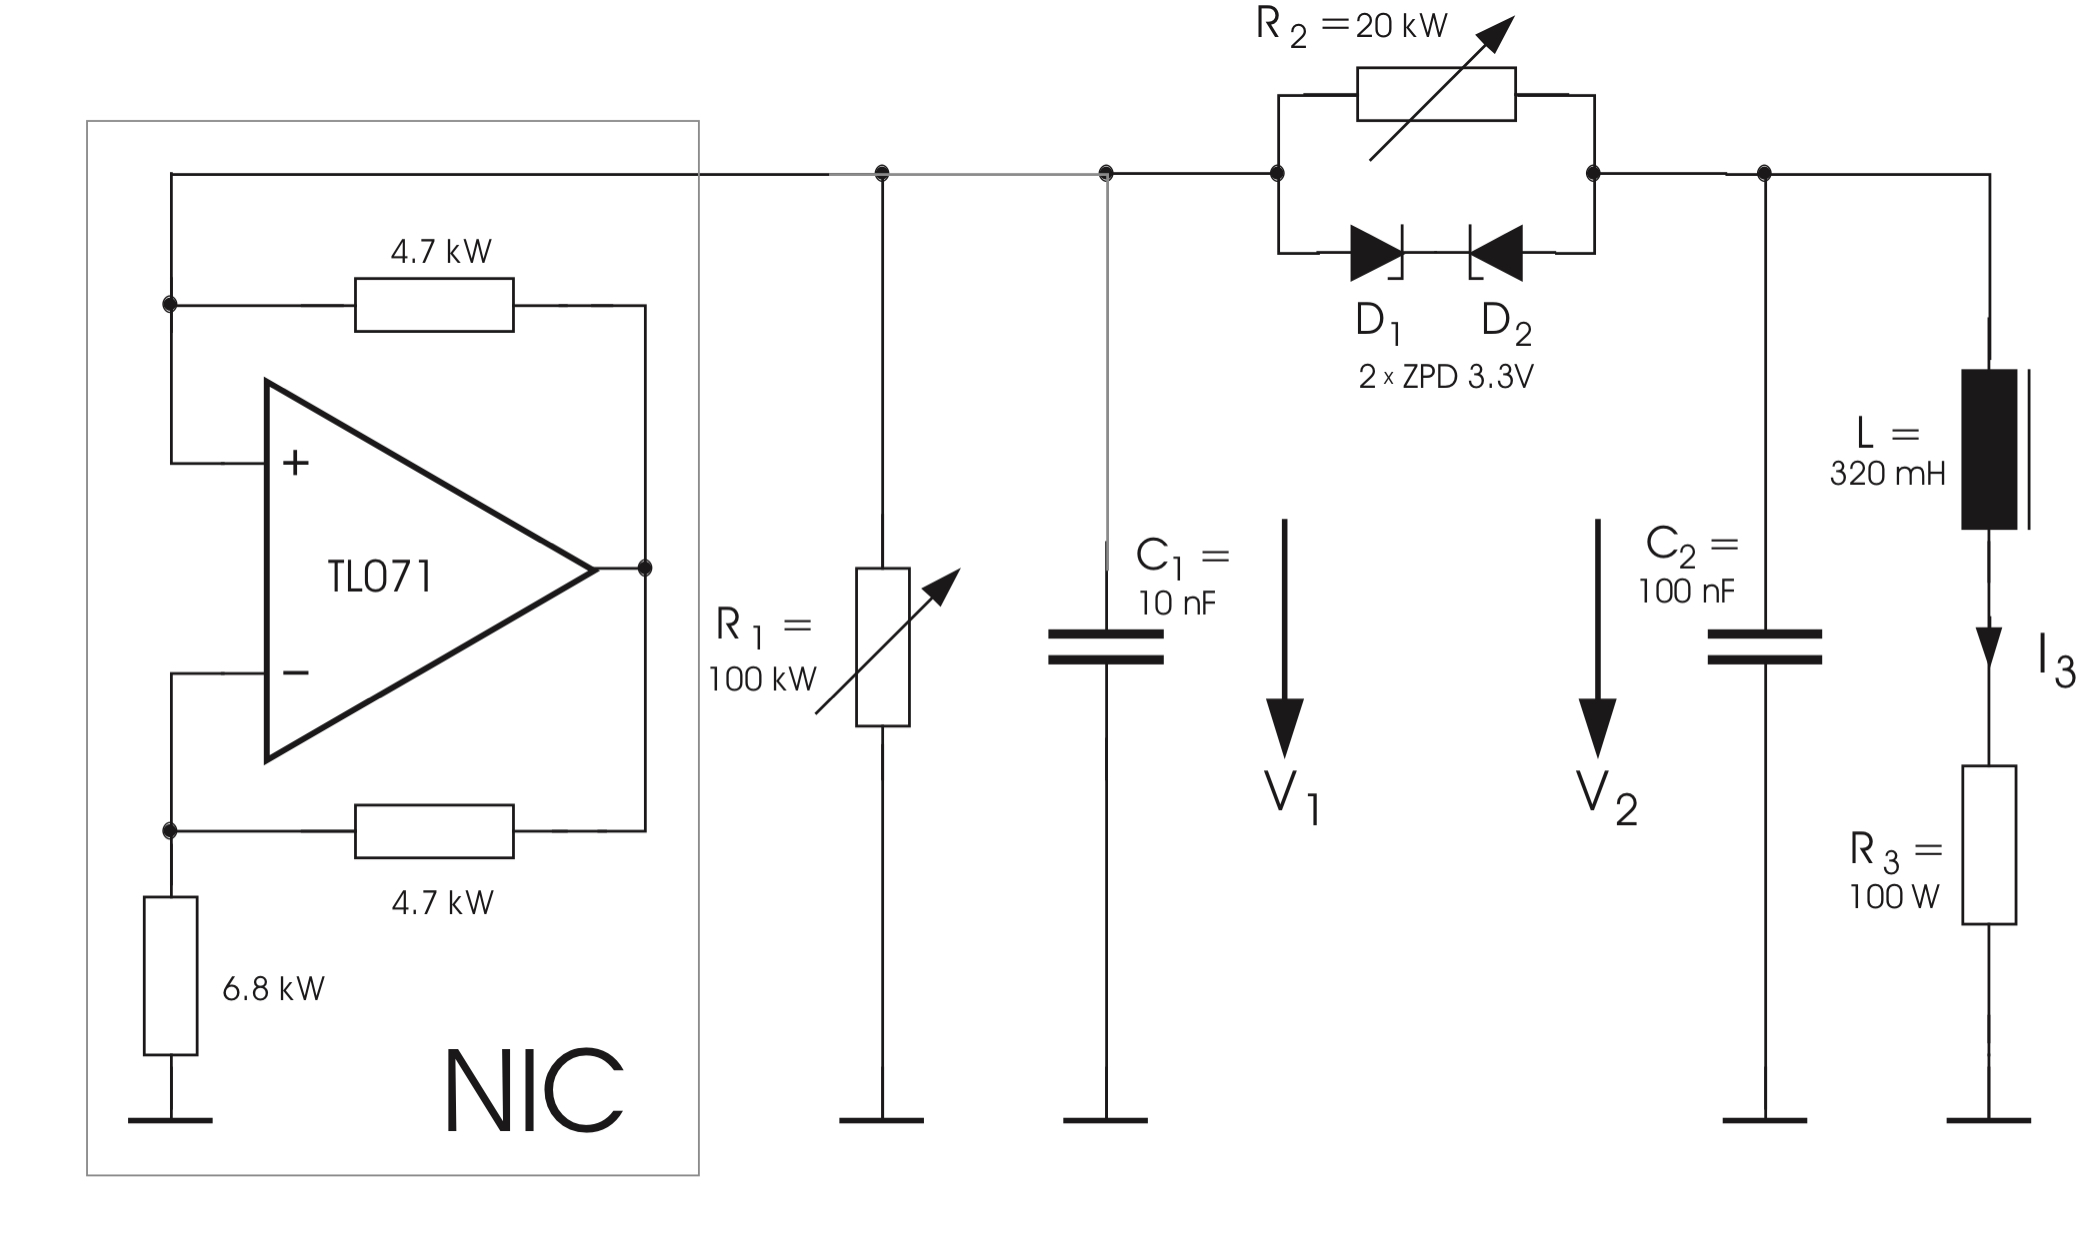
\includegraphics[scale=0.15]{ShinrOsziSp.jpeg}
    \label{fig:shinrikiSp}
    \caption{Schaltplan des Shinriki-Oszilator}
\end{figure}
% TODO: #25 Aufbau Shinriki @PaulSchwanitz

\section{Versuchsdurchführung}
\label{sec:durchfuehrung}

% Einbindung des Protokolls als pdf (mit Seitenzahl etc.)
% Erste Seite mit Überschrift
%\includepdf[pages = 1, landscape = false, nup = 1x1, scale = \skalierung , pagecommand={\thispagestyle{empty}\chapter{Protokoll}}]
%            {03-Protokoll/Protokoll.pdf}
% Restliche Seiten richtig skaliert
%\includepdf[pages = -, landscape = false, nup = 1x1, scale = \skalierung , pagecommand={}]
%            {03-Protokoll/Protokoll.pdf}